\chapter{Biological Subsystems}
\label{ch:biological-subsystems}

\epigraph{Nothing in biology makes sense except in the light of evolution.}{--- Theodosius Dobzhansky}

\lettrine[lines=2]{T}{he tumor microenvironment} is governed by three tightly coupled biological subsystems that together determine the trajectory of disease progression and treatment response. First, glucose metabolism creates spatial resource gradients through the Warburg effect, establishing zones of nutrient abundance near vasculature and depletion around tumor masses; these gradients shape both tumor proliferation capacity and immune effector function. Second, a 16-gene DNA mutation system drives clonal evolution, enabling tumor cells to accumulate mutations that enhance proliferation, suppress apoptosis, and critically, evade immune recognition through loss of antigen presentation machinery. Third, circulating sex hormones---estrogen, testosterone, and progesterone---modulate the strength and character of the immune response through 17 distinct effect channels, producing the pronounced sex disparities observed clinically in renal cell carcinoma. These subsystems interact bidirectionally: glucose gradients impose the selective pressure under which genetic evolution proceeds, the resulting mutations determine each tumor cell's visibility to immune surveillance, and the hormonal milieu sets the immunological context within which recognition and killing occur. The following sections present each subsystem's biological basis, mathematical formulation, and computational implementation before examining how they couple to produce emergent dynamics.

%% ====================================================================
%% SECTION 1: GLUCOSE MICROENVIRONMENT
%% ====================================================================
\section{Glucose Microenvironment}
\label{sec:glucose-microenvironment}

%% --------------------------------------------------------------------
\subsection{Biological Motivation}
\label{sec:glucose-bio}

\begin{figure}[htbp]
\centering
\adjustbox{max width=0.85\textwidth, max height=0.7\textheight}{% Warburg Effect: Normal vs Cancer Cell Metabolism
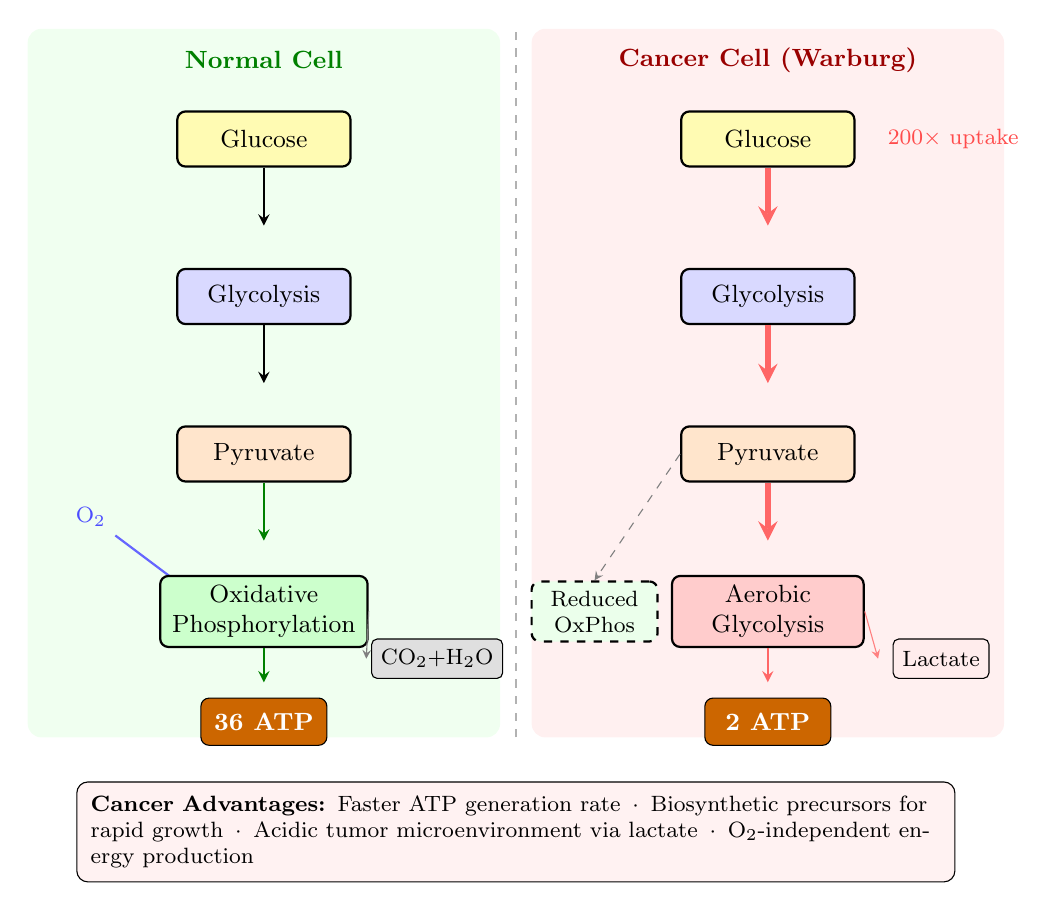
\begin{tikzpicture}[
  box/.style={draw, rounded corners=3pt, minimum width=2.2cm, minimum height=0.7cm,
              align=center, font=\small, thick},
  atp/.style={draw, rounded corners=3pt, font=\small\bfseries, text=white, fill=orange!80!black,
              minimum width=1.6cm, minimum height=0.6cm, align=center},
  byproduct/.style={draw, rounded corners=2pt, font=\footnotesize, fill=gray!25,
                    minimum height=0.5cm, align=center},
  arrow/.style={->, >=stealth, thick},
  fatarrow/.style={->, >=stealth, line width=2pt},
]

% Background panels
\fill[green!6, rounded corners=5pt] (-3.2, -0.4) rectangle (2.8, 8.6);
\fill[red!6, rounded corners=5pt] (3.2, -0.4) rectangle (9.2, 8.6);

% Panel headers
\node[font=\small\bfseries, green!50!black] at (-0.2, 8.2) {Normal Cell};
\node[font=\small\bfseries, red!60!black] at (6.2, 8.2) {Cancer Cell (Warburg)};

% Dividing line
\draw[dashed, gray!60, thick] (3.0, -0.4) -- (3.0, 8.6);

% === Normal Cell (left column, centered at x=0) ===
\node[box, fill=yellow!30] (gn) at (-0.2, 7.2) {Glucose};
\draw[arrow] (gn) -- ++(0, -1.1);

\node[box, fill=blue!15] (gly_n) at (-0.2, 5.2) {Glycolysis};
\draw[arrow] (gly_n) -- ++(0, -1.1);

\node[box, fill=orange!20] (pyr_n) at (-0.2, 3.2) {Pyruvate};
\draw[arrow, green!50!black] (pyr_n) -- ++(0, -1.1);

% O2 input
\node[font=\footnotesize, blue!70] (o2) at (-2.4, 2.4) {O$_2$};
\draw[arrow, blue!60] (o2) -- (-1.2, 1.5);

\node[box, fill=green!20, text width=2.4cm] (oxphos) at (-0.2, 1.2) {Oxidative\\Phosphorylation};
\draw[arrow, green!50!black] (oxphos) -- ++(0, -0.9);

\node[atp] (atp_n) at (-0.2, -0.2) {36 ATP};

\node[byproduct] at (2.0, 0.6) {CO$_2$+H$_2$O};
\draw[->, >=stealth, thin, gray] (oxphos.east) -- (1.1, 0.6);

% === Cancer Cell (right column, centered at x=6.2) ===
\node[box, fill=yellow!30] (gc) at (6.2, 7.2) {Glucose};
\node[font=\footnotesize, red!70, right] at (7.6, 7.2) {200$\times$ uptake};
\draw[fatarrow, red!60] (gc) -- ++(0, -1.1);

\node[box, fill=blue!15] (gly_c) at (6.2, 5.2) {Glycolysis};
\draw[fatarrow, red!60] (gly_c) -- ++(0, -1.1);

\node[box, fill=orange!20] (pyr_c) at (6.2, 3.2) {Pyruvate};
\draw[fatarrow, red!60] (pyr_c) -- ++(0, -1.1);

\node[box, fill=red!20, text width=2.2cm] (aero) at (6.2, 1.2) {Aerobic\\Glycolysis};
\draw[arrow, red!60] (aero) -- ++(0, -0.9);

\node[atp] (atp_c) at (6.2, -0.2) {2 ATP};

% Lactate
\node[byproduct, fill=pink!30] (lac) at (8.4, 0.6) {Lactate};
\draw[->, >=stealth, thin, red!50] (aero.east) -- (7.6, 0.6);

% Dashed branch to reduced OxPhos
\node[box, fill=green!8, font=\footnotesize, dashed, minimum width=1.6cm] (rox) at (4.0, 1.2) {\footnotesize Reduced\\OxPhos};
\draw[->, >=stealth, dashed, gray] (pyr_c.west) -- (rox.north);

% === Bottom advantages box (full width) ===
\node[draw, rounded corners=4pt, fill=red!5, text width=10.8cm, align=left, font=\footnotesize,
      inner sep=5pt] at (3.0, -1.6) {%
\textbf{Cancer Advantages:}\enspace
Faster ATP generation rate \,$\cdot$\,
Biosynthetic precursors for rapid growth \,$\cdot$\,
Acidic tumor microenvironment via lactate \,$\cdot$\,
O$_2$-independent energy production};

\end{tikzpicture}
}
\caption{The Warburg effect: metabolic competition in the tumor microenvironment.}
\label{fig:warburg_effect}
\end{figure}

The metabolic landscape of the tumor microenvironment plays a decisive role in determining immune-tumor interactions. As depicted in Figure~\ref{fig:warburg_effect}, Otto Warburg observed that tumor cells preferentially metabolize glucose through aerobic glycolysis, resulting in substantially elevated glucose uptake (up to 200-fold compared to normal tissue). This metabolic competition between tumor cells and infiltrating immune cells creates nutrient gradients that shape spatial organization, as regions surrounding tumor masses become nutrient-deprived. T cells and NK cells critically depend on glucose availability for cytotoxic activity --- when glucose is scarce, T cell proliferation is impaired, IFN-$\gamma$ production decreases, and cytotoxic granule release is diminished. In the absence of direct cell-cell contact, immune cells can follow glucose concentration gradients as a proxy for proximity to functional vasculature and viable tissue, providing a chemotactic fallback behavior.

The spatial distribution evolves dynamically as the simulation progresses (Figure~\ref{fig:glucose_dynamics}).

\begin{figure}[htbp]
\centering
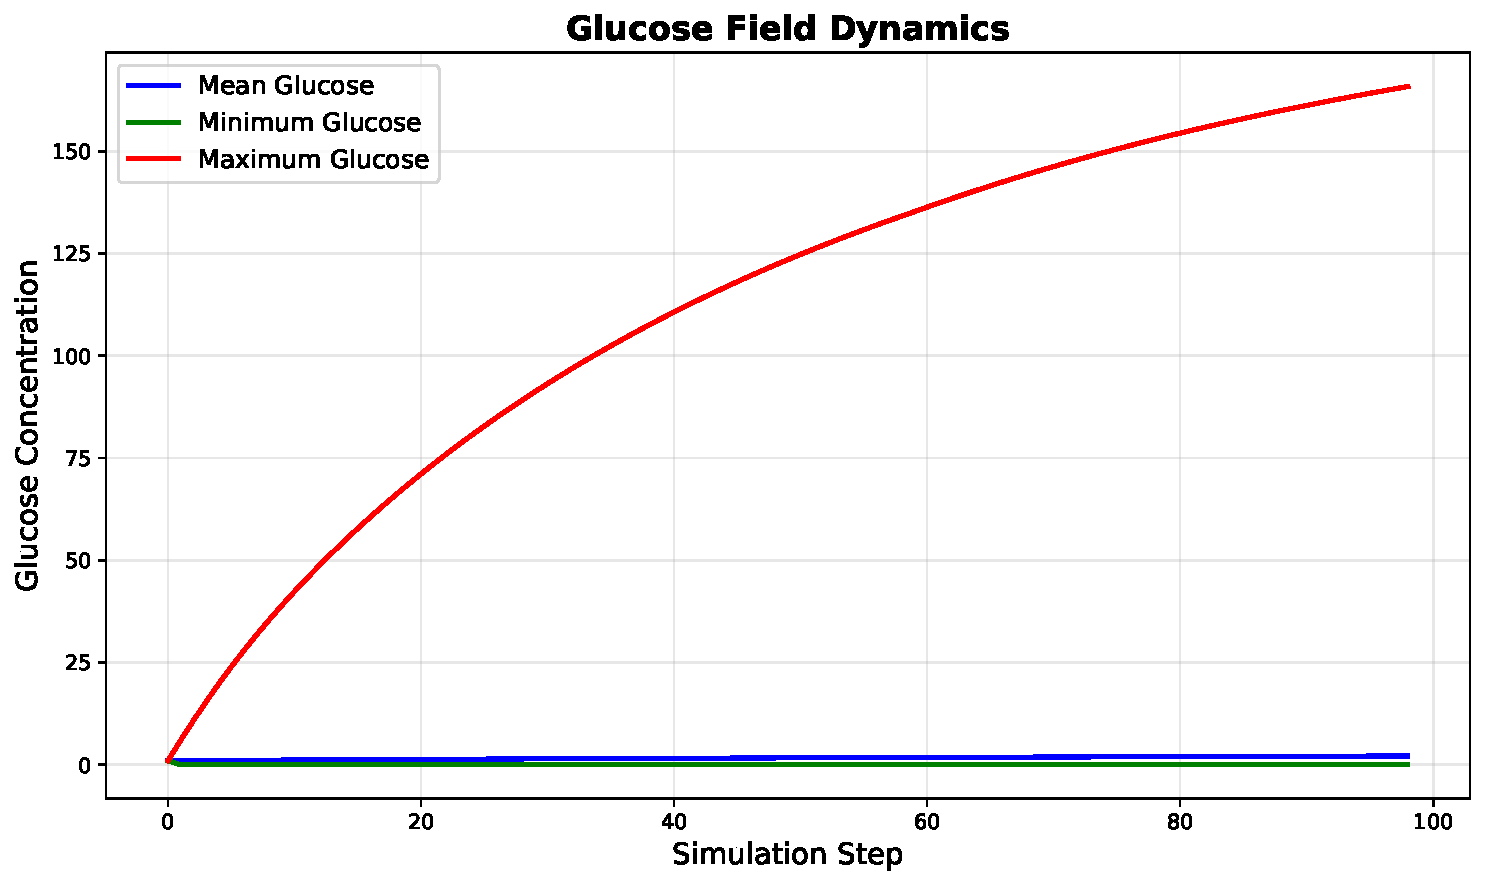
\includegraphics[width=0.85\textwidth]{figures/glucose_dynamics.pdf}
\caption{Glucose field dynamics showing depletion zones around tumor masses and gradients from blood vessels.}
\label{fig:glucose_dynamics}
\end{figure}

Blood vessels serve as point sources, the field diffuses according to Fick's law, and cellular agents consume glucose at position-dependent rates (Figure~\ref{fig:glucose_system}).

\begin{figure}[htbp]
\centering
\adjustbox{max width=0.85\textwidth, max height=0.7\textheight}{% Glucose System Block Diagram
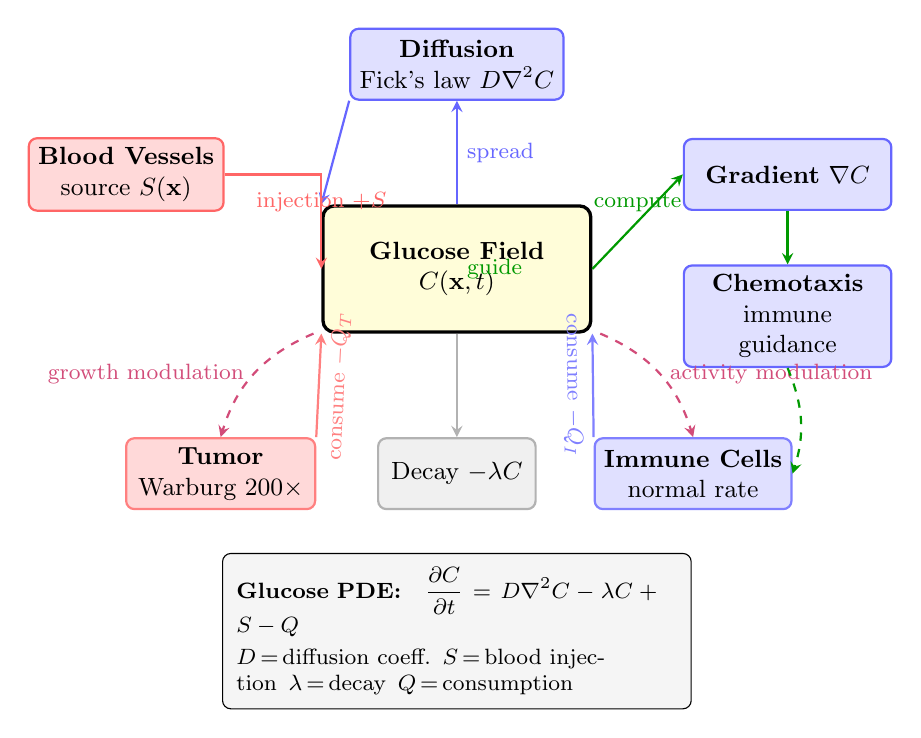
\begin{tikzpicture}[
  block/.style={draw, rounded corners=3pt, minimum width=2.4cm, minimum height=0.9cm,
                align=center, font=\small, thick},
  field/.style={draw, rounded corners=4pt, minimum width=3.4cm, minimum height=1.6cm,
                align=center, font=\small, thick, fill=yellow!15, line width=1.2pt},
  src/.style={block, fill=red!15, draw=red!60},
  proc/.style={block, fill=blue!12, draw=blue!60},
  cons/.style={block, fill=orange!15, draw=orange!60},
  arrow/.style={->, >=stealth, thick},
  dasharrow/.style={->, >=stealth, thick, dashed, purple!70},
]

% Central field
\node[field] (F) at (0, 0) {\textbf{Glucose Field}\\$C(\mathbf{x},t)$};

% Top: Diffusion
\node[proc] (diff) at (0, 2.6) {\textbf{Diffusion}\\Fick's law $D\nabla^2 C$};
\draw[arrow, blue!60] (F.north) -- (diff.south) node[midway, right, font=\footnotesize] {spread};
\draw[arrow, blue!60] (diff.south west) -- (F.north west);

% Left: Blood Vessels source
\node[src] (bv) at (-4.2, 1.2) {\textbf{Blood Vessels}\\source $S(\mathbf{x})$};
\draw[arrow, red!60] (bv.east) -- (F.west |- bv) -- (F.west)
  node[midway, above, font=\footnotesize] {injection $+S$};

% Right: Gradient & Chemotaxis
\node[proc, text width=2.4cm] (grad) at (4.2, 1.2) {\textbf{Gradient} $\nabla C$};
\node[proc, text width=2.4cm] (chem) at (4.2, -0.6) {\textbf{Chemotaxis}\\immune guidance};
\draw[arrow, green!60!black] (F.east) -- (grad.west) node[midway, above, font=\footnotesize] {compute};
\draw[arrow, green!60!black] (grad) -- (chem);

% Bottom-left: Tumor consumer
\node[cons, fill=red!15, draw=red!50] (tum) at (-3.0, -2.6) {\textbf{Tumor}\\Warburg 200$\times$};
\draw[arrow, red!50] (tum.north east) -- (F.south west)
  node[midway, below, sloped, font=\footnotesize] {consume $-Q_T$};

% Bottom-right: Immune consumer
\node[cons, fill=blue!12, draw=blue!50] (imm) at (3.0, -2.6) {\textbf{Immune Cells}\\normal rate};
\draw[arrow, blue!50] (imm.north west) -- (F.south east)
  node[midway, below, sloped, font=\footnotesize] {consume $-Q_I$};

% Below center: Decay
\node[proc, fill=gray!12, draw=gray!60, minimum width=2.0cm] (dec) at (0, -2.6) {Decay $-\lambda C$};
\draw[arrow, gray!60] (F.south) -- (dec.north);

% Dashed feedback arrows
\draw[dasharrow] (F.south west) ++(-0.1, 0) to[bend right=25]
  node[midway, left, font=\footnotesize, text=purple!70] {growth modulation} (tum.north);
\draw[dasharrow] (F.south east) ++(0.1, 0) to[bend left=25]
  node[midway, right, font=\footnotesize, text=purple!70] {activity modulation} (imm.north);

% Chemotaxis feedback
\draw[arrow, green!60!black, dashed] (chem.south) to[bend left=20] (imm.east)
  node[midway, right, font=\footnotesize] {guide};

% PDE equation box
\node[draw, rounded corners=3pt, fill=gray!8, inner sep=5pt, font=\footnotesize,
      text width=5.6cm, align=left] (pde) at (0, -4.6) {%
\textbf{Glucose PDE:}\quad
$\displaystyle\frac{\partial C}{\partial t} = D\nabla^2 C - \lambda C + S - Q$\\[2pt]
$D$\,=\,diffusion coeff.\enspace
$S$\,=\,blood injection\enspace
$\lambda$\,=\,decay\enspace
$Q$\,=\,consumption};

\end{tikzpicture}
}
\caption{Glucose system architecture showing the diffusion field, sources from blood vessels, and consumption by cellular agents.}
\label{fig:glucose_system}
\end{figure}

%% --------------------------------------------------------------------
\FloatBarrier
\subsection{Mathematical Formulation}
\label{sec:glucose-math}

The glucose concentration field $C(\mathbf{x}, t)$ evolves according to a reaction--diffusion equation derived from Fick's second law:

\begin{equation}
\label{eq:glucose-pde}
\frac{\partial C}{\partial t} = D\,\nabla^2 C \;-\; \lambda\,C \;+\; S(\mathbf{x}) \;-\; Q(\mathbf{x}),
\end{equation}

\noindent where $C(\mathbf{x}, t)$ is the glucose concentration, $D$ is the diffusion coefficient (\param{w\_glucose\_\allowbreak diffusion}, default $0.1$), $\lambda$ is the natural decay rate (\param{w\_glucose\_decay}, default $0.01$), $S(\mathbf{x})$ is the source term (glucose injection from blood vessels), and $Q(\mathbf{x})$ is the consumption term (uptake by tumor and immune cells).

The continuous Laplacian $\nabla^2 C$ is discretized on a regular 3D Cartesian grid using the standard 6-connected stencil, implemented as a 3D convolution using \param{scipy.\allowbreak ndimage.\allowbreak convolve}. The diffusion equation is advanced using explicit Euler integration with stability condition $D < 1/6 \approx 0.167$; the default $D = 0.1$ remains safely within the stable regime. Neumann (zero-flux) boundary conditions are enforced, corresponding to no glucose flux through simulation domain walls.

\paragraph{Source and Consumption Models.}

Blood vessel agents inject glucose at their grid positions at rate $r_{\text{source}}$ (\param{w\_glucose\_\allowbreak source\_rate}, default 5.0) per step. Tumor cells consume glucose reflecting the Warburg effect at rate $r_{\text{tumor}}$ (\param{w\_glucose\_\allowbreak tumor\_consumption}, default 2.0), while immune cells consume at lower rate $r_{\text{immune}}$ (\param{w\_glucose\_\allowbreak immune\_consumption}, default 0.5).

Tumor cell proliferation probability is modulated by glucose availability: $f_{\text{glucose}} = \min(1.0, C(\mathbf{x}_t) \cdot w_{\text{growth\_sensitivity}})$, and immune cell kill rates are similarly scaled: $f_{\text{immune}} = \min(1.0, C(\mathbf{x}_i) \cdot w_{\text{immune\_sensitivity}})$. When glucose is abundant ($C \geq 1.0$), activities proceed at full rate; as glucose drops below 1.0, functions are proportionally suppressed.

%% --------------------------------------------------------------------
\FloatBarrier
\subsection{Gradient and Chemotaxis}
\label{sec:glucose-chemotaxis}

The glucose gradient is computed using central finite differences, and for agent movement on the integer grid, the continuous gradient is converted to discrete step directions using the sign function. Immune cells that implement glucose chemotaxis (\texttt{CytotoxicTCell}, \texttt{MacrophageM1}, \texttt{DendriticCell}, \texttt{NaturalKiller}) employ a fallback strategy where they first attempt to move towards nearby tumor cells, and if no target is found, they move in the direction of increasing glucose concentration with probability $p_{\text{chemo}}$ (\texttt{w\_glucose\_chemotaxis\_strength}, default 0.3).

%% --------------------------------------------------------------------
\FloatBarrier
\subsection{Implementation}
\label{sec:glucose-impl}

The glucose system is encapsulated in the \texttt{GlucoseField} class, which stores concentrations as a 3D NumPy array (\texttt{float64}, initialized to 1.0). Each simulation step proceeds through injection (blood vessels deposit glucose at their grid positions), diffusion (discrete Laplacian convolution with Euler integration), and decay (multiplication by $1 - \lambda$). Agent-level consumption occurs within each agent's \texttt{step()} method via vectorized NumPy operations, and the class exposes aggregate statistics (mean, min, max) for tracking metabolic dynamics.

Mean glucose levels decline as tumor mass grows; minimum concentrations approach zero in regions of highest tumor density (Figure~\ref{fig:glucose_timeseries}).

\begin{figure}[htbp]
\centering
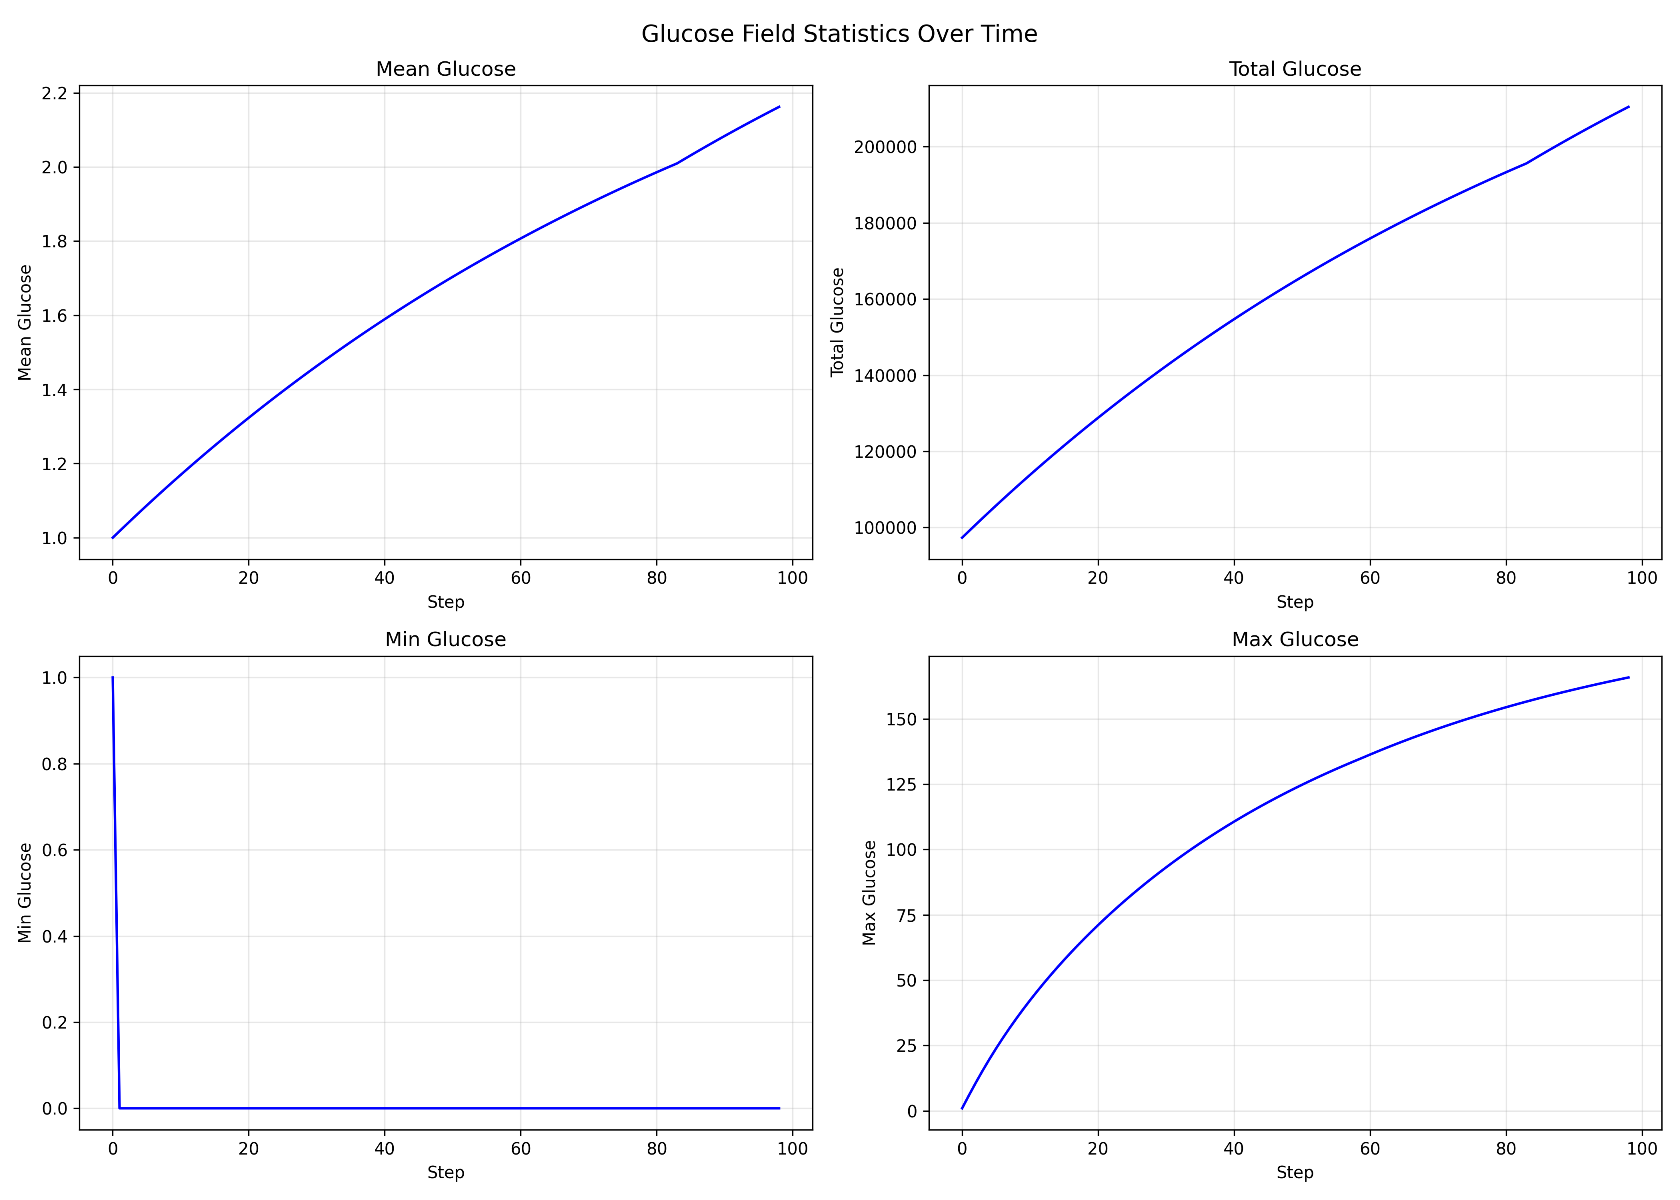
\includegraphics[width=0.85\textwidth]{figures/glucose_timeseries.pdf}
\caption{Glucose concentration time series (mean, min, max) reflecting injection, consumption, and diffusion.}
\label{fig:glucose_timeseries}
\end{figure}

The 3D field structure (Figure~\ref{fig:glucose_field_3d}) produces clearly delineated metabolic territories that constrain agent behavior.

\begin{figure}[htbp]
\centering
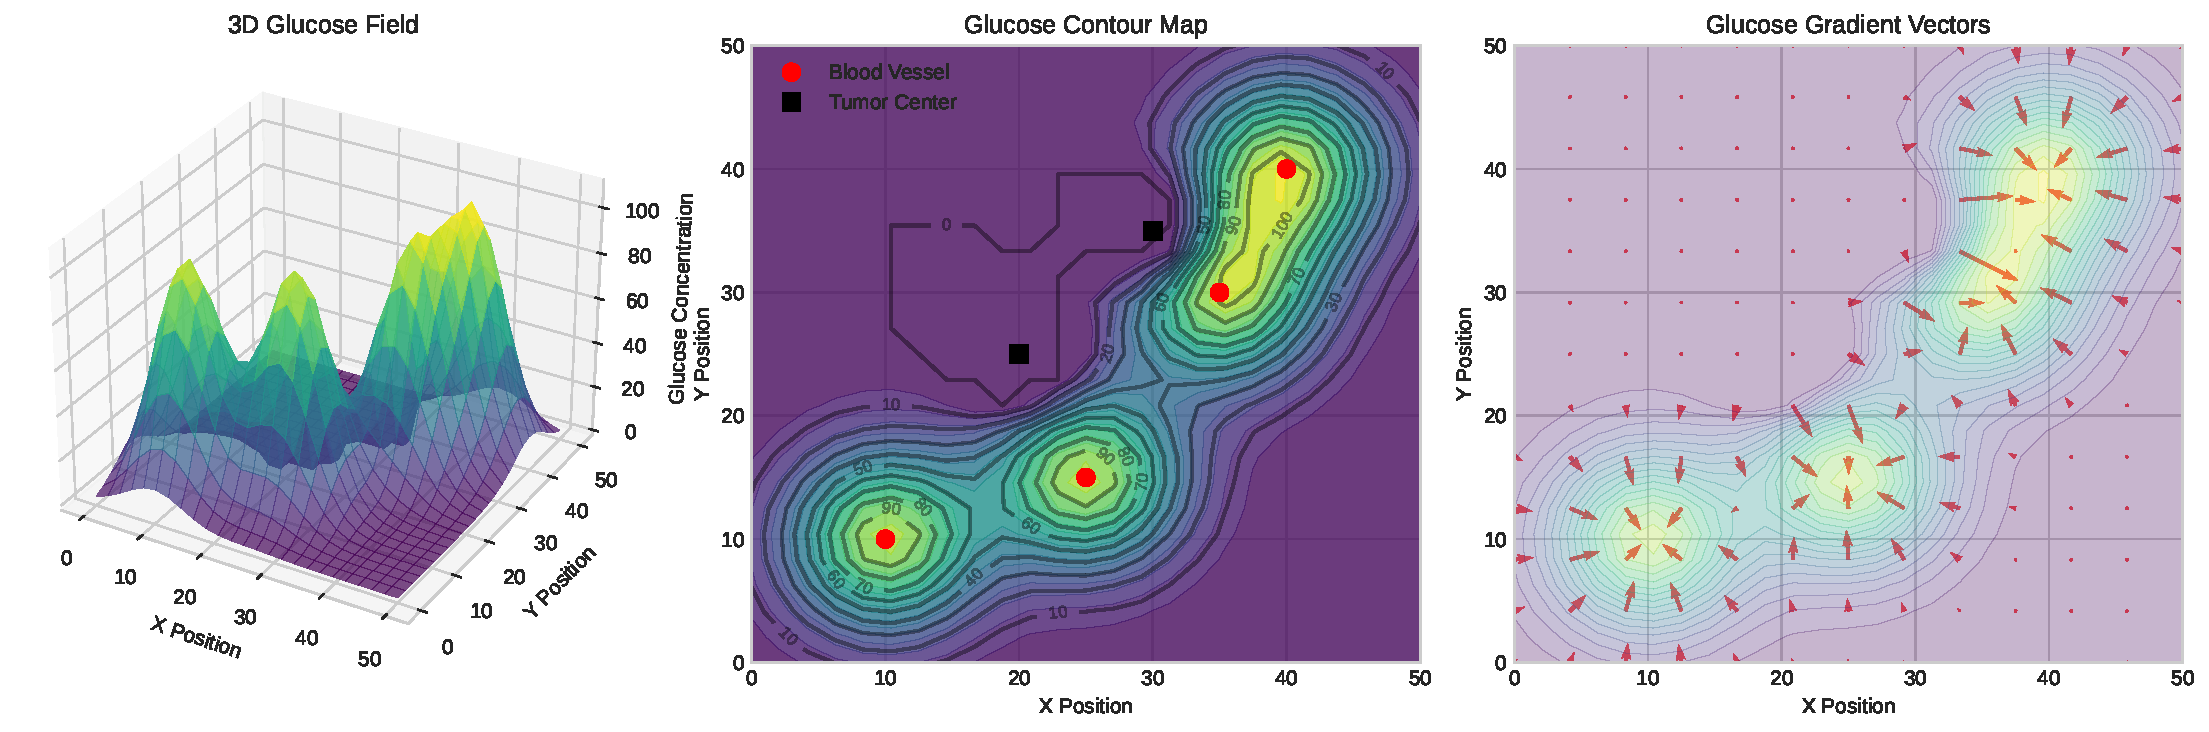
\includegraphics[width=0.85\textwidth]{figures/glucose_field_3d.pdf}
\caption{3D glucose field: high concentrations (yellow) near blood vessels, depletion (blue) near tumor masses.}
\label{fig:glucose_field_3d}
\end{figure}

The circular coupling between injection, diffusion, consumption, and chemotaxis is summarized in Figure~\ref{fig:glucose_system_cycle}.

\begin{figure}[htbp]
\centering
\adjustbox{max width=0.85\textwidth, max height=0.7\textheight}{% Glucose Dynamics Cycle Diagram
\begin{tikzpicture}[
  every node/.append style={font=\small},
  src/.style={ellipse, draw=orange!70, fill=orange!15, minimum width=2.2cm,
              minimum height=0.9cm, align=center, thick},
  proc/.style={rectangle, rounded corners=3pt, draw=green!60!black, fill=green!12,
               minimum width=2.2cm, minimum height=0.9cm, align=center, thick},
  cons/.style={rectangle, rounded corners=3pt, draw=red!60, fill=red!12,
               minimum width=2.2cm, minimum height=0.9cm, align=center, thick},
  eff/.style={rectangle, rounded corners=3pt, draw=blue!60, fill=blue!12,
              minimum width=2.2cm, minimum height=0.9cm, align=center, thick},
  arrow/.style={->, >=stealth, thick, shorten >=2pt, shorten <=2pt},
]

% 7 nodes arranged in a circle (radius ~3.2cm, starting from top, clockwise)
% Angles: 90, 38.6, -12.9, -64.3, -115.7, -167.1, 141.4
\def\R{3.2}

\node[src]  (bv)   at (90:\R)     {Blood\\[-1pt]Vessels};
\node[proc] (inj)  at (38.6:\R)   {Glucose\\[-1pt]Injection};
\node[proc] (diff) at (-12.9:\R)  {Spatial\\[-1pt]Diffusion};
\node[cons] (tum)  at (-64.3:\R)  {Tumor\\[-1pt]Consumption};
\node[cons] (star) at (-115.7:\R) {Immune\\[-1pt]Starvation};
\node[eff]  (grad) at (-167.1:\R) {Concentration\\[-1pt]Gradient};
\node[eff]  (chem) at (141.4:\R)  {Immune\\[-1pt]Chemotaxis};

% Cycle arrows
\draw[arrow, orange!70]       (bv)   -- (inj);
\draw[arrow, green!60!black]  (inj)  -- (diff);
\draw[arrow, green!60!black]  (diff) -- (tum);
\draw[arrow, red!60]          (tum)  -- (star);
\draw[arrow, red!60]          (star) -- (grad);
\draw[arrow, blue!60]         (grad) -- (chem);
\draw[arrow, blue!60]         (chem) -- (bv);

% Center label
\node[font=\small\bfseries, align=center, text=gray!70!black] at (0, 0) {Glucose\\Dynamics\\Cycle};

% Subtle annotation labels
\node[font=\footnotesize, orange!70!black, above=1pt] at (bv.north) {source};
\node[font=\footnotesize, red!60!black, below=1pt] at (tum.south) {Warburg effect};
\node[font=\footnotesize, blue!60!black, left=1pt] at (grad.west) {spatial signal};

\end{tikzpicture}
}
\caption{Glucose system cycle illustrating the circular flow of glucose dynamics in the tumor microenvironment.}
\label{fig:glucose_system_cycle}
\end{figure}

%% ====================================================================
%% SECTION 2: DNA AND MUTATION SYSTEM
%% ====================================================================
\section{DNA and Mutation System}
\label{sec:dna-mutation-system}

The gene-level representation used by tumor cells encodes 16 cancer-relevant genes, supports codon-level translation, introduces mutations during cell division with genomic-instability-dependent rates, and derives phenotypic parameters that govern tumor behavior and immune evasion.

%% --------------------------------------------------------------------
\subsection{Gene Model}
\label{sec:gene-model}

Each tumor cell carries a DNA object encoding 16 genes chosen for their relevance to renal cell carcinoma immunology, spanning antigen presentation, immune checkpoint signaling, DNA repair, tumor suppression, and oncogenic proliferation.

The 16 genes span five functional categories: \emph{antigen presentation} (MHC, B2M, TAP1, TAP2, JAK1, JAK2)---mutations in these genes reduce surface peptide display and enable immune evasion; \emph{immune checkpoint} (CD274/PD-L1)---overexpression engages PD-1 on T~cells; \emph{DNA repair} (BRCA1)---dysfunction increases genomic instability and mutation rate; \emph{tumor suppression} (TP53, RB1, CDKN2A, APC)---loss removes cell cycle checkpoints and apoptosis triggers; and \emph{oncogenes} (MYC, RAS, EGFR, HER2)---gain-of-function drives proliferation.

\begin{figure}[htbp]
\centering
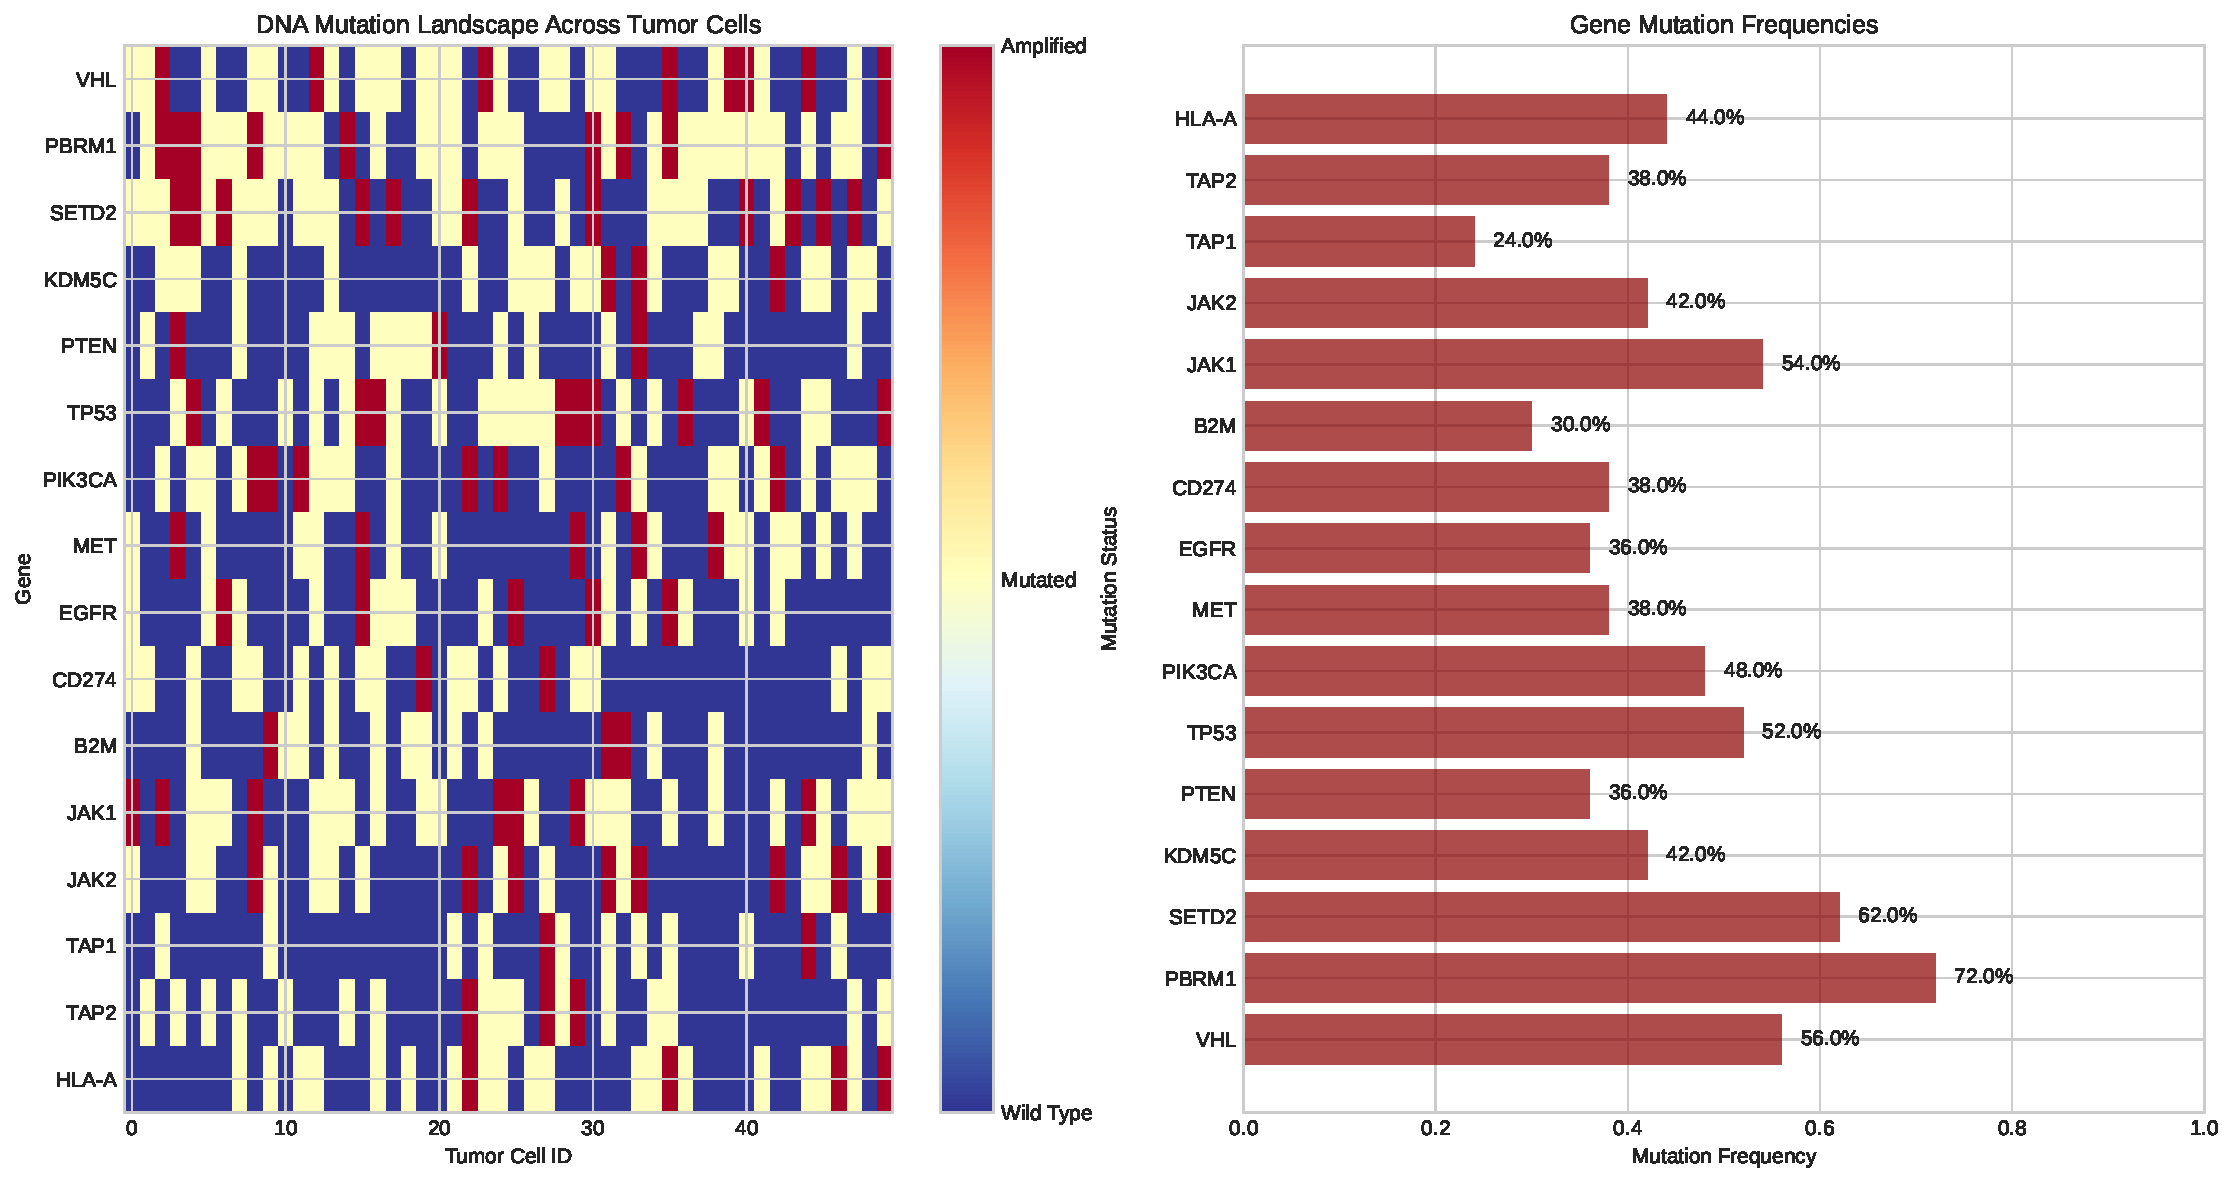
\includegraphics[width=0.85\textwidth]{figures/dna_mutation_heatmap.pdf}
\caption{DNA mutation heatmap across the 16 genes; color intensity indicates mutation severity.}
\label{fig:dna_mutation_heatmap}
\end{figure}

Each gene occupies a defined region within a synthetic DNA sequence assembled by concatenating spacer, promoter (including TATA box), coding region with codon-encoded wildtype protein, and stop codon, using full 64-codon translation.

%% --------------------------------------------------------------------
\FloatBarrier
\subsection{Mutation Mechanics}
\label{sec:mutation-mechanics}

Mutations accumulate through injected mutations at initialization and stochastic point mutations during DNA duplication.  Genomic instability is controlled by BRCA1 mutation status, with mutation rate scaling as $\mu = (s_{BRCA1})^{\max(1, e_{BRCA1})} \times 0.05$.  Initial mutations are sex-dependent: males start with 3 BRCA1 mutations, females with 1.  This asymmetry compounds over time---higher initial BRCA1 dysfunction increases the per-nucleotide mutation rate during subsequent divisions, producing greater clonal diversity and faster immune evasion in male tumors.

%% --------------------------------------------------------------------
\FloatBarrier
\subsection{Gene Expression and Phenotypic Effects}
\label{sec:gene-expression}

\begin{figure}[htbp]
\centering
\adjustbox{max width=0.85\textwidth, max height=0.7\textheight}{% Tumor Cell State Machine Diagram
\begin{tikzpicture}[scale=0.9, every node/.style={scale=0.9}]

% Define states
\tikzstyle{state}=[draw, circle, minimum size=2cm, text width=1.8cm, text centered]
\tikzstyle{decision}=[draw, diamond, minimum size=1.5cm, text width=1.3cm, text centered, aspect=2]
\tikzstyle{action}=[draw, rectangle, rounded corners, minimum width=2cm, minimum height=1cm, text centered]

% States
\node[state, fill=tumorcell!20] (quiescent) at (0,0) {
    \textbf{Quiescent}\par
    Low metabolism\par
    Dormant
};

\node[state, fill=tumorcell!40] (active) at (6,0) {
    \textbf{Active}\par
    High glucose\par
    consumption
};

\node[state, fill=tumorcell!60] (dividing) at (12,0) {
    \textbf{Dividing}\par
    DNA replication\par
    Mitosis
};

\node[state, fill=tumorcell!80] (aggressive) at (6,-4) {
    \textbf{Aggressive}\par
    Angiogenesis\par
    Invasion
};

\node[state, fill=red!80] (apoptotic) at (0,-8) {
    \textbf{Apoptotic}\par
    Cell death\par
    pathway
};

% Decision points
\node[decision, fill=yellow!50] (growth_check) at (3,2) {
    Growth\par
    signals?
};

\node[decision, fill=yellow!50] (division_check) at (9,2) {
    Ready to\par
    divide?
};

\node[decision, fill=yellow!50] (stress_check) at (9,-2) {
    Stress\par
    signals?
};

\node[decision, fill=yellow!50] (immune_check) at (3,-6) {
    Immune\par
    attack?
};

% Actions
\node[action, fill=green!30] (consume_glucose) at (6,3) {
    Consume\par
    Glucose
};

\node[action, fill=green!30] (duplicate) at (12,3) {
    Create\par
    Daughter Cell
};

\node[action, fill=orange!30] (angiogenesis) at (9,-5) {
    Promote\par
    Angiogenesis
};

\node[action, fill=purple!30] (pd_l1) at (3,-3) {
    Express\par
    PD-L1
};

% Transitions with conditions
\draw[thick, ->] (quiescent) to[bend left=20] node[above] {\tiny Nutrients available} (growth_check);
\draw[thick, ->] (growth_check) -- node[right] {\tiny Yes} (active);
\draw[thick, ->] (growth_check) to[bend left=30] node[left] {\tiny No} (quiescent);

\draw[thick, ->] (active) -- (consume_glucose);
\draw[thick, ->] (consume_glucose) -- (active);

\draw[thick, ->] (active) -- node[above] {\tiny DNA replication complete} (division_check);
\draw[thick, ->] (division_check) -- node[right] {\tiny Yes} (duplicate);
\draw[thick, ->] (duplicate) -- (dividing);

\draw[thick, ->] (dividing) to[bend left=40] node[above] {\tiny Division complete} (active);

\draw[thick, ->] (division_check) to[bend left=20] node[left] {\tiny No} (active);

\draw[thick, ->] (active) to[bend right=20] node[right] {\tiny Hypoxia/stress} (stress_check);
\draw[thick, ->] (stress_check) -- node[right] {\tiny Yes} (aggressive);
\draw[thick, ->] (stress_check) to[bend right=20] node[below] {\tiny No} (active);

\draw[thick, ->] (aggressive) -- (angiogenesis);
\draw[thick, ->] (angiogenesis) -- (aggressive);

\draw[thick, ->] (aggressive) to[bend left=20] node[below] {\tiny Oxygen restored} (active);

% Immune evasion
\draw[thick, ->] (active) to[bend right=30] (pd_l1);
\draw[thick, ->] (aggressive) to[bend left=30] (pd_l1);
\draw[thick, ->] (pd_l1) to[bend right=20] (immune_check);

\draw[thick, ->] (immune_check) to[bend left=20] node[left] {\tiny Evaded} (active);
\draw[thick, ->] (immune_check) -- node[below] {\tiny Killed} (apoptotic);

% Death pathways
\draw[thick, ->, red] (quiescent) to[bend right=60] node[left] {\tiny DNA damage} (apoptotic);
\draw[thick, ->, red] (active) to[bend right=30] node[left] {\tiny Immune killing} (apoptotic);
\draw[thick, ->, red] (dividing) to[bend left=60] node[right] {\tiny Mitotic arrest} (apoptotic);
\draw[thick, ->, red] (aggressive) to[bend left=30] node[right] {\tiny Treatment} (apoptotic);

% Self loops for waiting states
\draw[thick, ->] (quiescent) to[loop above] node[above] {\tiny Wait} (quiescent);
\draw[thick, ->] (dividing) to[loop above] node[above] {\tiny Complete mitosis} (dividing);

% Title
\node[text width=14cm, text centered] at (6,6) {
    \Large\textbf{Tumor Cell State Machine and Decision Tree}
};

% Legend
\node[draw, rounded corners, fill=white, text width=3.5cm] at (-3,3) {
    \textbf{Legend}\par
    \textcolor{tumorcell}{\textbullet} Cellular States\par
    \textcolor{yellow!50}{\textbullet} Decision Points\par
    \textcolor{green!30}{\textbullet} Actions\par
    \textcolor{red}{—} Death Pathways
};

% Parameter influences
\node[draw, rounded corners, fill=blue!10, text width=4cm] at (15,1) {
    \textbf{Key Parameters}\par
    • \texttt{tumour\_growth\_effect}\par
    • \texttt{tumour\_apoptosis\_effect}\par
    • \texttt{angiogenesis\_effect}\par
    • DNA mutation profile\par
    • Glucose availability\par
    • Blood access
};

% DNA influence indicator
\node[draw, star, fill=dna, text=white] (dna) at (12,-2) {DNA};
\draw[thick, ->, dashed] (dna) -- (division_check) node[midway, right] {\tiny Mutation effects};
\draw[thick, ->, dashed] (dna) -- (pd_l1) node[midway, below] {\tiny CD274 expression};

\end{tikzpicture}}
\caption{State machine diagram of tumor cell lifecycle.}
\label{fig:tumor_cell_state_machine}
\end{figure}

The lifecycle of a tumor cell---from quiescence through proliferation, immune interaction, and potential apoptosis---is governed by a state machine shown in Figure~\ref{fig:tumor_cell_state_machine}. Each gene's phenotypic contribution is determined by promoter expression (TATA motif count) and mutation score (Levenshtein distance from wildtype protein). The DNA system computes five aggregate phenotypic parameters:

\textbf{Antigen Presentation Chance}: $p_{AP} = \max(0, 6 - \frac{\sum_{g \in \{MHC,JAK1,JAK2,B2M,TAP1,TAP2\}} e_g \cdot s_g}{6})$ represents the tumor cell's ability to present antigens, with mutations reducing this probability for immune evasion.

\textbf{Checkpoint Inhibition Chance}: $p_{CPI} = e_{CD274} \cdot s_{CD274}$ determined by PD-L1 gene, with higher mutated expression increasing T cell checkpoint engagement probability.

\textbf{Genomic Instability}: Controls mutation rate during DNA duplication based on BRCA1 dysfunction level.

\textbf{Tumor Suppression Chance}: $p_{TS} = \frac{1}{3}\sum_{g \in \{TP53,RB1,CDKN2A\}} e_g \cdot (1-s_g)$ with functional tumor suppressors increasing apoptosis probability.

\textbf{Extra Proliferation Chance}: $p_{EP} = \frac{1}{5}(\sum_{g \in \{MYC,RAS,EGFR,HER2\}} e_g \cdot (1-s_g) + e_{APC} \cdot s_{APC})$ capturing oncogene-driven growth.

%% --------------------------------------------------------------------
\FloatBarrier
\subsection{Neoantigen Generation}
\label{sec:neoantigens}

Neoantigens---novel peptide fragments produced by somatic mutations---are the molecular interface between tumor evolution and immune surveillance.  Biologically, mutated proteins are degraded, loaded onto MHC~I molecules via the TAP1/TAP2 pathway, and displayed on the cell surface for T~cell recognition.  In the model, neoantigens are represented as 10-mer subsequences extracted from each translated mutated protein, while self-antigens are computed from wildtype sequences to establish immune tolerance.  T~cell receptors recognize neoantigens through Hamming distance matching between antigen hashes and receptor values: successful recognition requires that the antigen is classified as non-self and that $d_H$ falls within a configurable threshold.  This abstraction preserves the essential properties that immune recognition is both specific (only sufficiently similar antigens trigger a response) and stochastic (dependent on the receptor repertoire sampled from the T~cell population).

%% ====================================================================
%% SECTION 3: SEX HORMONE SYSTEM
%% ====================================================================
\section{Sex Hormone System}
\label{sec:sex-hormone-system}

The sex hormone subsystem models the immunomodulatory effects of estrogen, testosterone, and progesterone on the tumor microenvironment. Sex-specific differences in hormone profiles produce distinct immune dynamics, contributing to the well-documented sex disparity in RCC incidence and treatment response.

%% --------------------------------------------------------------------
\subsection{Biological Basis}
\label{sec:hormone-bio}

Renal cell carcinoma exhibits a pronounced sex disparity---males are affected approximately twice as often as females, yet treatment efficacy varies significantly between sexes---driven in part by the distinct immunomodulatory profiles of the three hormones modeled here.

Estrogen is biphasic: low-to-moderate concentrations promote Th1 responses via ER$\alpha$ signaling, while high concentrations shift toward Th2 dominance and Treg differentiation.  Testosterone is broadly immunosuppressive, reducing Th1 proliferation and accelerating thymic involution.  Progesterone is dose-dependent, ranging from negligible to strongly immunosuppressive at high concentrations.

%% --------------------------------------------------------------------
\FloatBarrier
\subsection{Hormone Agent Model}
\label{sec:hormone-agent}

Sex hormones are discrete agents that diffuse through the grid, interact with nearby immune cells, and decay over time. They are spawned from blood vessel positions with sex-specific probabilities (Table~\ref{tab:hormone-spawn}), perform biased random walks with drift away from vasculature, and are removed upon grid exit (effective lifespan $\approx$50 steps).

\begin{table}[H]
\centering
\caption{Hormone spawn probabilities by patient sex.}
\label{tab:hormone-spawn}
\begin{tabular}{lccc}
\toprule
\textbf{Sex} & \textbf{Estrogen} & \textbf{Progesterone} & \textbf{Testosterone} \\
\midrule
Male   & 0.2 & 0.1 & 1.0 \\
Female & 0.9 & 0.8 & 0.2 \\
\bottomrule
\end{tabular}
\end{table}

%% --------------------------------------------------------------------
\FloatBarrier
\subsection{Hormone Effects on T Cells}
\label{sec:hormone-effects}

T cells detect sex hormones via the \param{perceive\_sex\_hormone()} method, maintaining dictionaries of perceived hormone levels that decay by 10\% per step.  The 17 effect channels (enumerated in Table~\ref{tab:hormonal-effects} in Appendix~\ref{ch:appendix-params}) span cytotoxic modulation, proliferation, apoptosis, activation, differentiation, Th1/Th2-specific proliferation, five cytokine axes (IL-4, IL-6, IL-13, IFN-$\gamma$, TNF-$\alpha$), MHC~I/II upregulation, CD28 costimulation, and checkpoint engagement (CTLA-4, PD-1).  Perceived hormone levels are normalized to $[0,1]$ and mapped to concentration regimes (low $<0.33$, medium $0.33$--$0.66$, high $\geq 0.66$), with effects weighted by hormone-specific importance: $w_{\text{estrogen}} = 0.45$, $w_{\text{testosterone}} = 0.30$, $w_{\text{progesterone}} = 0.25$.

%% --------------------------------------------------------------------
\FloatBarrier
\subsection{Sex Drift}
\label{sec:sex-drift}

The model implements population-level sex drift that adjusts CD8$^+$ na\"ive T~cell populations based on patient sex, reflecting testosterone's effect on thymic output.  Over $n = 15$ steps, a per-step factor $f = 1 + \sigma \cdot d_{\max}/n$ (with $d_{\max} = 0.25$, $\sigma = +1$ for males, $-1$ for females) drives duplication or removal, producing approximately $\pm$25\% population change.  The resulting temporal evolution of hormone concentrations is shown in Figure~\ref{fig:hormone_dynamics}.

\begin{figure}[htbp]
\centering
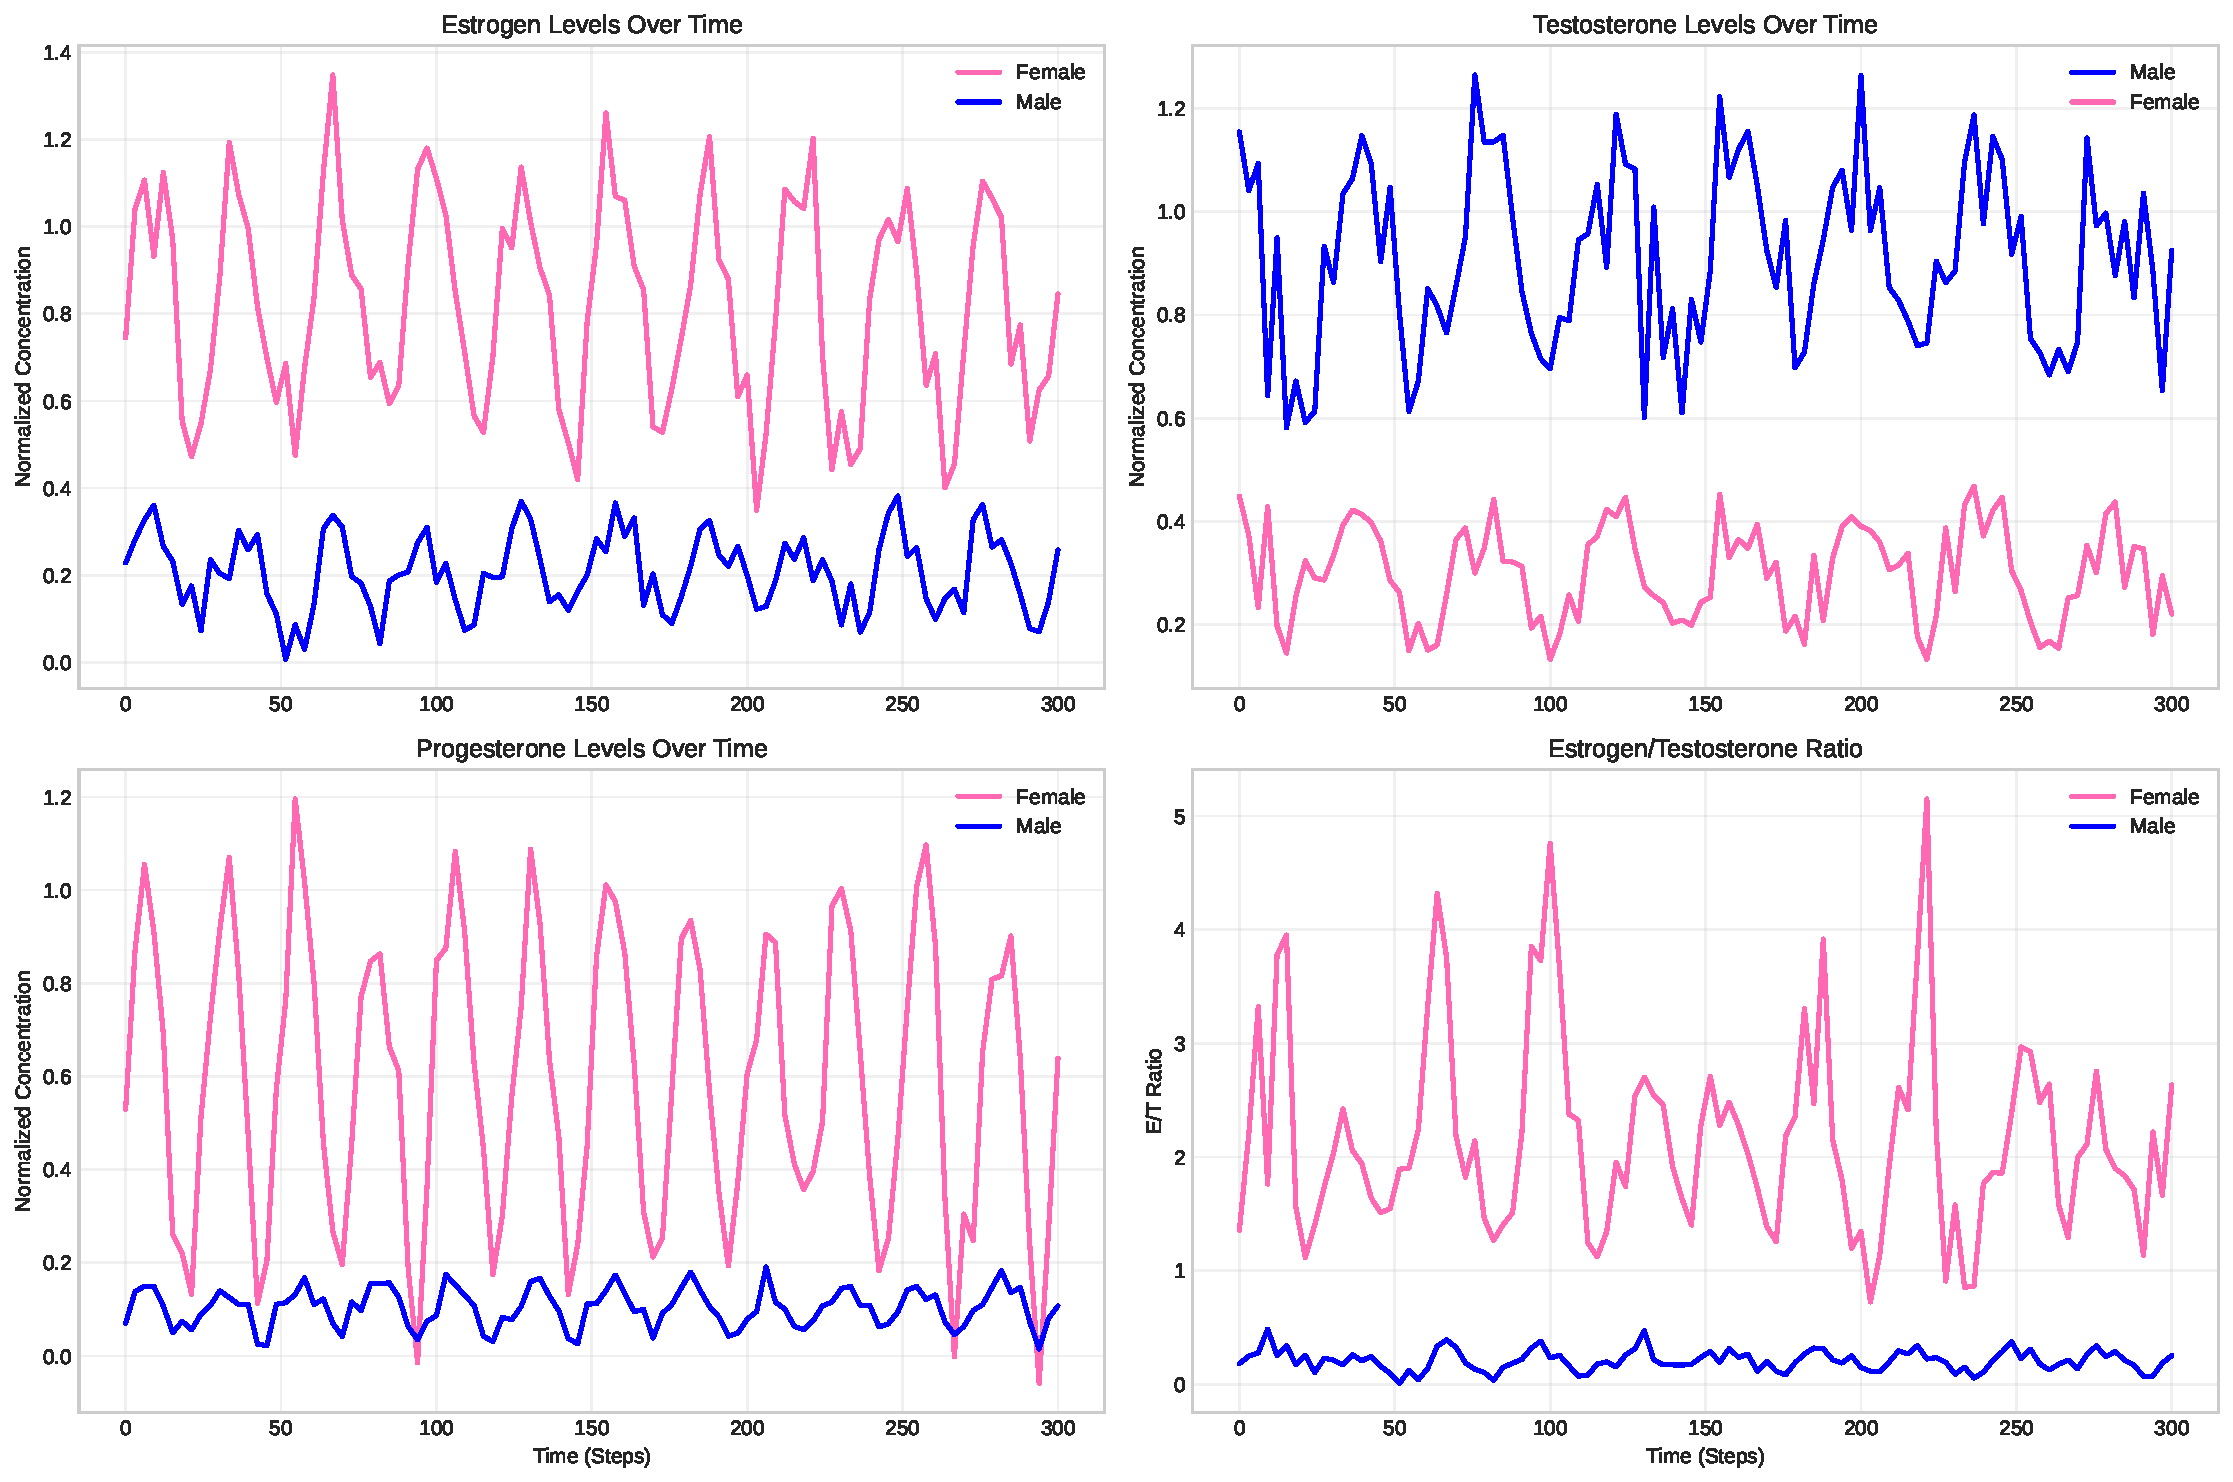
\includegraphics[width=0.85\textwidth]{figures/hormone_dynamics.pdf}
\caption{Sex hormone dynamics over time for estrogen, testosterone, and progesterone.}
\label{fig:hormone_dynamics}
\end{figure}

%% ====================================================================
%% CHAPTER SUMMARY
%% ====================================================================
These three subsystems---glucose metabolism, DNA mutation, and sex hormones---interact bidirectionally to produce the emergent tumor-immune dynamics that the treatment system, described in the next chapter, aims to disrupt.
